% TODO - WORK IN PROGRESS
\subsection{Attack Description} % ~ 2.5 to 3 pages (including subsections)
\label{sec:exp:description}

% TODO intro

The following paragraphs give a detailed description of the main steps to realize such an attack. Therefore we first need to look more precisely at the functional principle of smart light bulbs. Further we have a look at how smooth brightness changes are achieved and how we actually get data out of the received signal.\newline

%write about brightness change frequency, why high sampling frequency is needed, Human eye threshold; mention parts in python program ... 

% TODO ?? talk about Short-time Fourier transform in corresponding section -> To illustrate the temporal change of the frequency spectrum of a signal.

\subsubsection{Contorlling Smart Light Bulbs.} 
% --> describe components of smart LEDs, how they work, controller communication
Smart light bulbs consist of three main components: (1) a RF receiver, (2) a processiong unit and (3) LEDs and LED drivers.
The communication with the controller is ensured through the \textit{RF receiver} and relies on the \textit{ZigBee~Light~Link}~(ZLL) protocol. The received commands are further forwarded to the \textit{processing unit} which interprets the processed signal and controls the LED by modulating the pulse width. The PWM allows the different dimming factors. When sending a brightness change command via the Hue API, this automatically forces the processing unit to generate the corresponding PWM signal. The PWM is sent to the LED drivers which further turn the LEDs on and off at a very fast rate such that those changes in the duty cycle cannot be seen by the human eye. Since Hue comes with 255 brightness levels which need to be differentiated smoothly, a PWM with a frequency around 20 KHz is used \cite{Ronen:2016:EFAIDCSL}. 

% TODO: for the following 2 sections to complete need to discuss what we now actually see and used sampling rate, which pics we want to use etc
\subsubsection{Crafting PWM Signal.}
% --> describe how fast changes are achieved, frequency output with light sensor, collection of signal with picoscope
% 10 MS/s = 10 MHz

% TODO fill in concrete values
Because of the great amount of brightness levels, we had to measure very small off periods of about xxx ns. This could be done with the described light sensor as well as the picoscope, since the light sensor's output is around 800 KHz, as can be seen in Figure \ref{fig:plot-140-135}, which we can sample at 10 MS/s with our picoscope.

\begin{figure}[h]
	\centering
	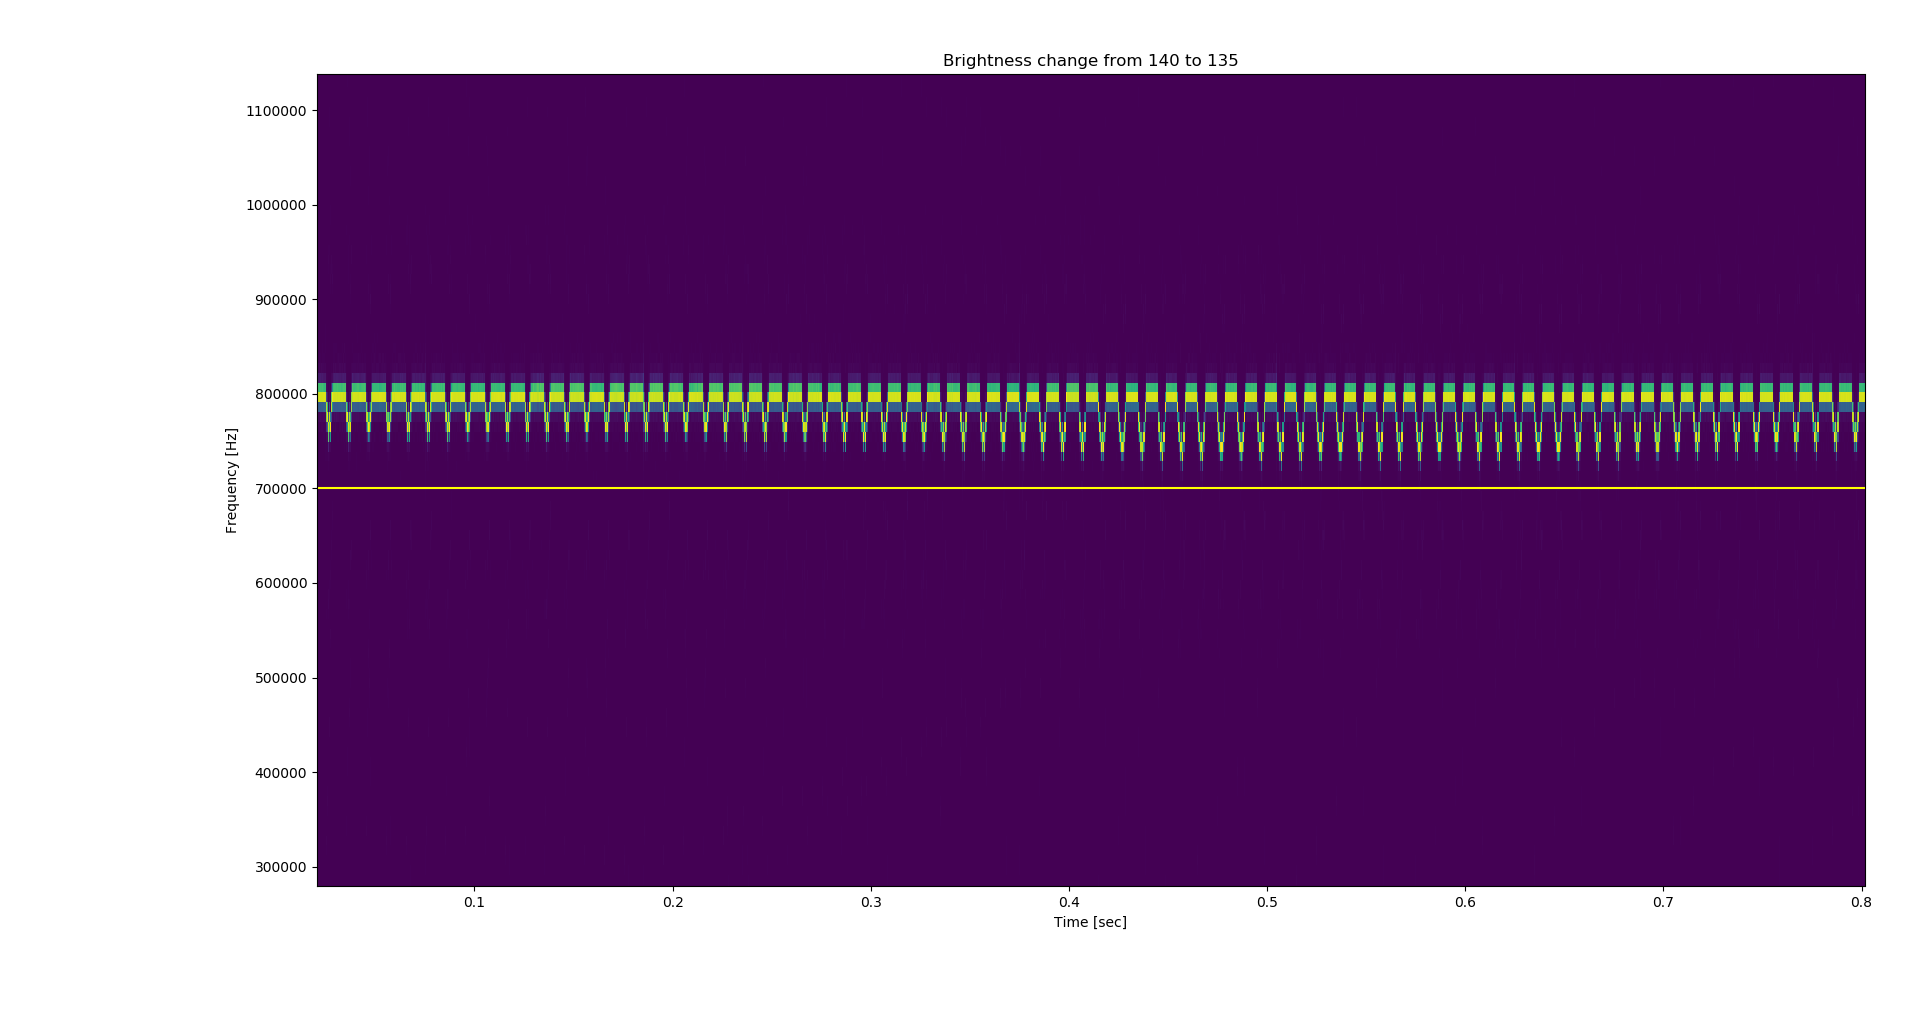
\includegraphics[width=14cm]{img/Plot_140_135.png}
	\caption{Brightness change from 140 to 135 sampled at 10 MS/s}
	\label{fig:plot-140-135}
\end{figure}

\subsubsection{Getting Data.}
% --> describe analysis of signal
